\documentclass[11pt]{article}

%%% XeLaTeX Font Definitions

\usepackage{titlesec}
\usepackage{titling}
\usepackage{xunicode}
\usepackage{fontspec,xltxtra,xunicode}
\usepackage[table,xcdraw]{xcolor}
\defaultfontfeatures{Mapping=tex-text}
\usepackage{bigints}
\usepackage{booktabs}
\usepackage{bm}

% Uncomment below to change default features 
%\setromanfont[Mapping=tex-text]{Hoefler Text}
%\setsansfont[Scale=MatchLowercase,Mapping=tex-text]{Gill Sans}
%\setmonofont[Scale=MatchLowercase]{Andale Mono}

% Specify different font for section headings
\newfontfamily\headingfont[]{Lucida Grande Bold}
\newfontfamily\titlefont[]{Optima}

\titleformat*{\section}{\Large\headingfont}
\titleformat*{\subsection}{\large\headingfont}
\titleformat*{\subsubsection}{\large\headingfont}
\renewcommand{\maketitlehooka}{\titlefont}

%%% Remove the "abstract" word before the abstract

\newcommand{\overbar}[1]{\mkern 1.5mu\overline{\mkern-1.5mu#1\mkern-1.5mu}\mkern 1.5mu}

\usepackage{abstract}
\renewcommand{\abstractname}{}    % clear the title
\renewcommand{\absnamepos}{empty} % originally center

%%% Actual Preamble

%\headheight=8pt
%\topmargin=3pt
%\textheight=624pt
%\textwidth=432pt
%\oddsidemargin=18pt
%\evensidemargin=18pt
\usepackage{amsmath}
\usepackage{amsfonts}
\usepackage{amssymb}
\usepackage{amsthm}
\usepackage{comment}
\usepackage{epsfig}
\usepackage{psfrag}
\usepackage{mathtools}

\DeclarePairedDelimiter{\ceil}{\lceil}{\rceil}

%\usepackage{sseq} (if you need to draw spectral sequences, please use this package, available at http://wwwmath.uni-muenster.de/u/tbauer/)
\usepackage{mathrsfs}
\usepackage{amscd}
\usepackage[all]{xy}
\usepackage{rotating}
\usepackage{lscape}
\usepackage{amsbsy}
\usepackage{verbatim}
\usepackage{moreverb}
\usepackage{mathdots}
\usepackage{setspace}
%\usepackage{eucal}
\usepackage{hyperref}
\usepackage{pgfplots}%http://www.ctan.org/pkg/pgfplots

\usepackage{listings}
\usepackage[margin=1in]{geometry}
\pagestyle{plain}
\theoremstyle{definition}
\newtheorem{theorem}{Theorem}%[section]
\newtheorem{prop}{Proposition}
\newtheorem{lemma}{Lemma}
\newtheorem{corollary}[theorem]{Corollary}
%\theoremstyle{definition}
\newtheorem{definition}{Definition}
\newtheorem{notation}{Notation}
\newtheorem{summary}{Summary}
\newtheorem{note}{Note}
\newtheorem{construction}[theorem]{Construction}
%\theoremstyle{remark}
\newtheorem{remark}{Remark}
\newtheorem{example}{Example}
\newtheorem{question}[example]{Question}
\DeclareMathOperator{\Aut}{Aut}
\DeclareMathOperator{\coeq}{coeq}
\DeclareMathOperator{\colim}{colim}
\DeclareMathOperator{\cone}{cone}
\DeclareMathOperator{\Der}{Der}
\DeclareMathOperator{\Ext}{Ext}
\DeclareMathOperator{\hocolim}{hocolim}
\DeclareMathOperator{\holim}{holim}
\DeclareMathOperator{\Hom}{Hom}
\DeclareMathOperator{\Iso}{Iso}
\DeclareMathOperator{\Map}{Map}
\DeclareMathOperator{\Tot}{Tot}
\DeclareMathOperator{\Tor}{Tor}
\DeclareMathOperator{\Spec}{Spec}
\newcommand{\TMF}{\mathit{TMF}}
\newcommand{\tmf}{\mathit{tmf}}
\newcommand{\Mell}{\mathcal M_{\mathit{ell}}}
\newcommand{\Mord}{\mathcal M_{\mathit{ell}}^{\mathit{ord}}}
\newcommand{\Mss}{\mathcal M_{\mathit{ell}}^{\mathit{ss}}}
\newcommand{\Mbar}{\overline{\mathcal M}_{\mathit{ell}}}
\newcommand{\Mfg}{\mathcal M_{\mathit{FGL}}}
\newcommand{\MU}{\mathit{MU}}
\newcommand{\MP}{\mathit{MP}}
\newcommand{\Lk}{L_{K(n)}}
\newcommand{\Lone}{L_{K(1)}}
\newcommand{\Ltwo}{L_{K(2)}}
\newcommand{\Sp}{\mathbf{Sp}}
\newcommand{\Eoo}{E_\infty}
\newcommand{\Aoo}{A_\infty}
\newcommand{\CP}{\mathbb{CP}^\infty}
\newcommand{\GL}{\mathit{GL}}
\newcommand{\gl}{\mathit{gl}}
\newcommand{\nn}{\nonumber}
\newcommand{\nid}{\noindent}
\newcommand{\ra}{\rightarrow}
\newcommand{\la}{\leftarrow}
\newcommand{\xra}{\xrightarrow}
\newcommand{\xla}{\xleftarrow}
\newcommand{\weq}{\xrightarrow{\sim}}
\newcommand{\cofib}{\rightarrowtail}
\newcommand{\fib}{\twoheadrightarrow}
 \newcommand{\xhdr}[1]{\vspace{2mm}\noindent{{\bf #1.}}}

\def\llarrow{   \hspace{.05cm}\mbox{\,\put(0,-2){$\leftarrow$}\put(0,2){$\leftarrow$}\hspace{.45cm}}}
\def\rrarrow{   \hspace{.05cm}\mbox{\,\put(0,-2){$\rightarrow$}\put(0,2){$\rightarrow$}\hspace{.45cm}}}
\def\lllarrow{  \hspace{.05cm}\mbox{\,\put(0,-3){$\leftarrow$}\put(0,1){$\leftarrow$}\put(0,5){$\leftarrow$}\hspace{.45cm}}}
\def\rrrarrow{  \hspace{.05cm}\mbox{\,\put(0,-3){$\rightarrow$}\put(0,1){$\rightarrow$}\put(0,5){$\rightarrow$}\hspace{.45cm}}}
\def\cA{\mathcal A}\def\cB{\mathcal B}\def\cc{\mathbf C}\def\cd{\mathbf D}
\def\ce{\mathcal E}\def\cf{\mathcal F}\def\cG{\mathcal G}\def\cH{\mathcal H}
\def\cI{\mathcal I}\def\cJ{\mathcal J}\def\cK{\mathcal K}\def\cL{\mathcal L}
\def\cM{\mathbf M}\def\cN{\mathcal N}\def\cO{\mathbf O}\def\cP{\mathcal P}
\def\cQ{\mathcal Q}\def\cR{\mathcal R}\def\cS{\mathcal S}\def\cT{\mathcal T}
\def\cU{\mathcal U}\def\cV{\mathcal V}\def\cW{\mathcal W}\def\cX{\mathcal X}
\def\cY{\mathcal Y}\def\cZ{\mathcal Z}
\def\AA{\mathbb A}\def\BB{\mathbb B}\def\CC{\mathbb C}\def\DD{\mathbb D}
\def\EE{\mathbb E}\def\FF{\mathbb F}\def\GG{\mathbb G}\def\HH{\mathbb H}
\def\II{\mathbb I}\def\JJ{\mathbb J}\def\KK{\mathbb K}\def\LL{\mathbb L}
\def\MM{\mathbb M}\def\NN{\mathbb N}\def\OO{\mathbb O}\def\PP{\mathbb P}
\def\QQ{\mathbb Q}\def\RR{\mathbb R}\def\SS{\mathbb S}\def\TT{\mathbb T}
\def\UU{\mathbb U}\def\VV{\mathbb V}\def\WW{\mathbb W}\def\XX{\mathbb X}
\def\YY{\mathbb Y}\def\ZZ{\mathbb Z}

\newcommand{\MFGL}{\mathcal M_{\mathit{FGL}}}
\newcommand{\calO}{{\mathcal O}}
\newcommand{\calC}{{\mathcal C}}
\newcommand{\set}{{\mathrm{Set}}}
\newcommand{\Deltab}{{\mathbf \Delta}}
\newcommand{\spet}{\mathrm{Spec}^\mathrm{\acute{e}t}}
\newcommand{\Z}{\mathbb Z}
\DeclareMathOperator{\Spf}{Spf}

\usepackage{fancyhdr}
\setlength{\headheight}{15.2pt}
\pagestyle{fancy}

\usepackage{booktabs}

\lhead{2016-17}
\chead{Information Theory}
\rhead{Manan Shah}

\graphicspath{{./figures/}}

\begin{document}
\title{\headingfont{Information Theory, Part II}}
\author{Manan Shah\\ \texttt{manan.shah.777@gmail.com} \\ The Harker School}
\maketitle
\begin{abstract}
This document contains lecture notes from Harker's Advanced Topics in Mathematics class in Information Theory II, taught by Dr. Anuradha Aiyer. This course is the second part of a two part offering that explores the basic concepts of Information Theory, as initially described by Claude Elwood Shannon at Bell Labs in 1948. These notes were taken using TeXShop and \LaTeX2$\epsilon$ and will be updated for each class. The reader is advised to note any errata at the source control repository \texttt{https://github.com/mananshah99/infotheory}.
\end{abstract}
\tableofcontents
\newpage

%% Notes start here

\section{Unit 1: Gambling}

We'll discuss the duality between the growth rate of investment (i.e. a horse race) and the entropy rate of the horse race and how the side information's financial value is tied to mutual information. 

\definition[Horse Race] We have $m$ horses in a race in which the $i$th horse wins with probability $p_i$. If horse $i$ wins, the payoff is $o_i$ for 1\footnote{There are two ways to describe a bet: either $a$ for 1 or $b$ to 1. The first notation indicates an exchange that happens prior to the race, and the latter indicates and exchange that happens post-race (although in both cases the horses are picked before the race). More concretely, $a$ for 1 indicates that if one places \$1 on a particular horse before the race, the payoff is \$a iff the horse wins and \$0 if the horse loses. $b$ to 1 indicates that one would pay \$1 after the race if a particular horse loses and win \$b if the horse wins. The equivalency between these scenarios is $b = a-1$.}. We'll assume that the gambler invests his wealth across all horses and doesn't hold on to any of his money. Specifically, $b_i$ is the fraction of wealth invested in horse $i$ where $b_i \geq 0$ and $\sum b_i = 1$. If horse $i$ wins, the gambler wins $o_i b_i$; this case occurs with probability $p_i$. The wealth at the end of the race is a random variable which we will attempt to maximize. 

\subsection{Repeated Gambling}

Define $S_n$ as the total growth in the gambler's wealth after $n$ races. We have $$S_n = \prod_{j=1}^n S(X_j) \qquad \text{and} \qquad S(X_j) = b(X_j) o(X_j)$$with $X$ representing the horse that wins (this changes between races). Here, $S(X_i)$ represents the factor by which the gambler's wealth grows. We can define the doubling rate of a race $W$ as $$E(\log S(X)) = \sum_{k=1}^m p_k \log (b_k o_k) = W(b, p)$$

\theorem Let race outcomes $X_1, X_2, X_3, \dots, X_n$ be identically and independently distributed $\sim p(x)$. The wealth of a gambler using betting strategy $b$ grows exponentially at the rate $W(b, p)$ such that $S_n = 2^{n W(b, p)}$.

\begin{proof}
Functions of independent random variables are also independent, so $\log S(X_1), \dots \log S(X_n)$ are i.i.d. From our earlier definition of $S_n$ we have $$\frac{1}{n} \log S_n = \frac{1}{n} \sum \log S(X_i)$$By the weak law of large numbers\footnote{See \texttt{http://mathworld.wolfram.com/WeakLawofLargeNumbers.html} for more information.}, this equates to $E(\log S(X)) = W(b, p)$. So we can conclude that $S_n =  2^{n W(b, p)}$ and the proof is complete. So if to maximize $S_n$, we'll need to maximize $W$. 
\end{proof}
\definition The optimum doubling rate over all choices of $b_i$ is $$W^*(p) = \max_b W(b, p) = \max_{b: \: b_i \geq 0, \: \sum b_i = 1} \sum_i p_i \log b_i o_i$$We must formally maximize $W(b, p)$ such that $\sum b_i = 1$. To do this, we'll apply Lagrange optimization. We have $$J(b) = \sum p_i \log b_i o_i + \lambda \sum b_i$$Taking the partial with respect to $b_i$ and setting it equal to 0, $$\frac{\partial J}{\partial b_i} = \frac{p_i}{b_i} + \lambda$$ where $i \in \{ 1 \dots m \}$. Solving for $b_i$ as a function of $p_i$ and $\lambda$, substituting the resulting value into the constraint $\sum b_i = 1$, and evaluating the differential expression with  $\lambda = -1$ results in $b_i = p_i$. Technically, we'd have to take the second derivative to prove that this is a maximum; this verification is left to the reader. 

\theorem $W^* = \sum p_i \log o_i - H(p)$

\begin{proof}
\begin{align*}
W(b, p) &= \sum p_i \log b_i o_i  \\
&= p_i \log \left( \frac{b_i}{p_i} \times p_i o_i \right) \\
&= \sum p_i \log o_i - H(p) - D(p || b)
\end{align*}
The last term, $D$, is known as relative entropy. It has some of the same properties of entropy, one of them being that $D \geq 0$. So,  $W(b, p) \leq \sum p_i \log o_i - H(p)$ with equality when $p = b$. 
\end{proof}

\subsection{Kullback-Liebler Divergence}

The function $D$, known as the relative entropy or Kullback-Liebler Divergence, is a measure of distance\footnote{This isn't technically a measure of distance as it doesn't satisfy the triangle inequality} between two distributions. If $p$ and $q$ are the two distributions, then $D(p || q)$ is a measure of inefficiency of assuming $q$ when the true distribution is $p$. The average code length for distribution $p$ is $H(p)$, but if we were to use the code for $q$ to encode $p$, then $H(p) + D(p||q)$ bits. 

\definition[Kullback-Liebler Divergence] The KL divergence $D(p||q)$ is expressed as $$D(p||q) = \sum_x p(x) \log \frac{p(x)}{q(x)} = E_x \left[ \log \frac{p(x)}{q(x)} \right] $$ where $0 \log 0/q = 0$ and $p \log p / 0 = \infty$. We can then write $I(X; Y) = \sum \sum p(x, y) \log \frac{p(x, y)}{p(x) p(y)}$ which is simplified to $D(p(x, y) || p(x) p(Y))$

\example $p(0) = 1-r, q(0) = 1-s, p(1) = r, q(1) = s$
$$D(p||q) = (1-r) \log \frac{1-r}{1-s} + r \log \frac{r}{s}$$ 
$$D(q||p) = (1-s) \log \frac{1-s}{1-r} + s \log \frac{s}{r}$$

\example Consider a case with two horses where horse 1 wins with probability $p_1$ and horse 2 wins with $p_2$. Assume even odds (2-for-1). (a) What is the optimal bet? (b) Doubling rate? (c) Resulting wealth? 

(a) The optimal bet is according to the probabilities of the horses, (b) The doubling rate is $1-H(p)$, and the resulting wealth (c) is $2^{n(1-H(p))}$

We further have that $W(b, p) = \sum p \log \frac{p_i}{r_i} - \sum p \log \frac{p}{b} = D(p || r) - D(p || b)$ where $r_i = 1/o_i$. The doubling rate is the difference between the distance of the bookie's estimates from the truth. The gambler only makes money when $b$ is closer than $r$. When the odds are $m$-for-1, we have $$W^*(p) = D(p || 1/m)= \log m - H(p)$$and $W^*(p) + H(p) = \log m$.
 
 \example Three horses run a race. A gambler offers 3-for-1 odds on each horse. Fair odds under the assumption that all horses are equally likely to win. $p = (1/2, 1/4, 1/4)$. (a) Expected wealth, (b) $b^*$, (c) $W^*$
 
(a) We have that $W(b) = \sum p_i \log b_i o_i = \sum p_i \log 3b$ since $o_i = 1/3$ due to fair odds. Therefore, $W(b) = \sum p_i \log 3 + \sum p_i \log b_i = \log 3 + \sum p_i \log b_i$. (b) $b^* = p = (1/2, 1/4/, 1/4)$ and (c) $W^* = W(b^*) - \log 3 - 3/2$. Note that we can solve (c) with the identity discussed above. 

\subsection{The Value of Side Information}

One measure is the increase in the doubling rate based on the information. We'll connect this increase with mutual information (as we connected $W^*$ with KL divergence and entropy before). Define $X \in \{1, 2, \dots m \}$ as the horse betting space, $p(x)$ as the probabilities associated with $1 \rightarrow m$, $o(x)$ for 1 odds, and $y$ as the side information. Furthermore, we have $\sum_x b(x|y)$ as the conditional betting depending on side information $y$ and $b(x|y)$ as the proportion of wealth bet on horse $x$ when $y$ is observed. Based on these definitions, we have $$W^*(X) = \max_{b(x)} \sum_x p(x) \log b(x) o(x)$$and given our side information, $$W^*(X|Y) = \max_{b(x|y)} \sum_{x, y} p(x, y) \log b(x|y) o(x)$$so we have $$\Delta W = W^*(X|Y) - W(X)$$

\theorem The increase doubling rate $\Delta W$ due to side information $Y$ for a horse race $X$ is $\Delta W = I(X; Y).$

\begin{proof}
We have that $b^*(x|y) = p(x|y)$. Since $W^*(X|Y) = \max_{b(x|y)} E(\log S)$\footnote{$S$ was defined earlier as the aggregate wealth}. This equates to $\max_{b(x|y)} \sum p(x, y) \log [o(x) b(x|y)]$. So, we have that $$W^*(X|Y) = \sum p(x,y) \log [p(x) p(x|y)] = \sum p(x) \log o(x) - H(X|Y)$$Without side information $W^* = \sum p(x) \log o(x) - H(X)$, so we have $\Delta W = \sum p(x) \log o(x) - H(X|Y) - [\sum p(x) \log o(x) - H(X)]$. Finally, we have $\Delta W = H(X) - H(X|Y) = I(X;Y)$.
\end{proof}

\example Given a three horse race $p = (1/2, 1/4, 1/4)$ with odds with respect to the false distribution $r_1, r_2, r_3 = (1/4, 1/4, 1/2)$ and $o_1, o_2, o_3 = (4, 4, 2)$\footnote{This is because $o_i = 1/r_i$ when determining the odds given the false distribution. ``Fair odds'' are defined such that $\sum 1/o_i = 1$}. Find (a) the entropy of the race and (b) $(b_1, b_2, b_3)$ such that compounded wealth $\rightarrow \infty$. 

The entropy of the race is easily calculated as $3/2$. It's intuitive that $b_i = o_i p_i$ so we have $(2, 1, 1/2)$, which we re-normalize to $(4/7, 2/7, 1/7)$. Our final $W = \sum p_i \log b_i o_i$. 

\example Let the distribution be $(p_1, p_2, p_3)$ with odds $o = (1, 1, 1)$ and wealth proportions $b = (b_1, b_2, b_3)$. $S_n \rightarrow 0$ exponentially. (a) Find the exponent, (b) $b^*$, and (c) What $p$ causes $S_n \rightarrow 0$ at the fastest rate. 

We always have that $b_i = \frac{p_i o_i}{\sum_i b_i}$, so we can write $b^* = p$. Furthermore, the exponent is simply the doubling rate $W = \sum p_i \log b_i o_i$, and the $P$ that causes $S_n \rightarrow 0$ most quickly is the one that maximizes $H(p)$ or $p = (1/3, 1/3, 1/3)$. 

\example Now assume you have the most common form of side information, the past performance of the horses. If the results of each successive horse race are independent, then this additional information will not reveal anything new about the race. Suppose instead that the races are dependent. How might we calculate $W^*(X_k | X_{k-1}, X_{k-2},..., X_1)$?\\

\noindent At the end of of $n$ races, $$S_n = \prod_i S(X_i)$$
Therefore,
\begin{align*}
\frac{1}{n} \mathrm{E}\left[\log{S_n}\right] &= \frac{1}{n} \sum_{i=1}^{n} \mathrm{E}\left[\log{S(X_i)}\right]\\
							        &= \frac{1}{n} \sum_{i=1}^{n} \left[\log{m} - H(X_i | ...)\right]\\
							  W^*&=  \log{m} - \frac{H(X_1, X_2,...,X_n)}{n}
\end{align*}
The term $\frac{H(X_1, X_2,...,X_n)}{n}$ can be thought of as the average entropy across all the races. 

\section{Unit 2: Statistics}

\subsection{Introduction}
Statistics considers two types of studies: observational and experimental. In an experimental study, treatments are assigned to subjects; this is not the case in observational studies. The first part of this topic was covered with traditional statistics worksheets involving the definition of $p$-values and statistical tests ($t$, $z$, etc.) A diagram that connects these concepts is as follows:

\begin{table}[ht]
\centering
\begin{tabular}{@{}lll@{}}
\toprule
Information Theory & Statistics            & Machine Learning      \\ \midrule
Source             & Observational Studies & Unsupervised Learning \\
Channel            & Experimental Studies  & Supervised Learning   \\ \bottomrule
\end{tabular}
\end{table}

We'll start by modeling the source, which has a distribution $Q$ and outputs the vector $X$. We will define a notion of $X$ as too ridiculous to have come from $Q$. It is incorrect to define the ridiculousness criterion as ``$\text{Prob}_Q(X)$ is small'' as looking at one event whose probability will almost always be small is insufficient.

\definition $X$ is ``too ridiculous'' to have originated from source $Q$ if and only if probability $\text{Prob}_Q$($X$ and its entire subsequent tail) is sufficiently small\footnote{Define $\epsilon$ as in traditional proofs to quantify this}. That is to say, given $X$ we can define 
\begin{equation*}
S_X = \{ X' \: | \: \text{Prob}_Q (X') \leq \text{Prob}_Q(X) \}
\end{equation*}We then have that $X$ is too ridiculous to have come from $Q$ if the probability $\text{Prob}_Q(S_X)$ is sufficiently small.

\definition[Confidence Interval] Given $X$, identify all $Q$s it may have originated from. The confidence interval\footnote{It's better to write this as a confidence region as opposed to a confidence interval if we're working in spaces of higher dimensionality than $\mathbb{R}^1$} is defined as $$\{Q \: | \: X \text{ is not too ridiculous to have originated from } Q\}$$

\definition[Hypothesis Test] Given hypothesis $Q$, find all $X$ that will allow for disproving $Q$. The rejection interval (or region) is defined as $$\{X \: | \: X \text{ is too ridiculous to have come from } Q \}$$

\subsection{Two Significant Theorems}

We'll discuss two important theorems that define the notions of $\text{Prob}_Q(X)$ and $\text{Prob}_Q(S)$.

\subsubsection{$\text{Prob}_Q(X)$}
Assume that we are given a source $Q$ that produces observed data outputs $X_1 \dots X_N$ (all abbreviated as the vector $X$) and that the values are identically and independently distributed. We will attempt to define the value $\text{Prob}_Q(X)$. If we were to histogram the vector $X$ (with the y axis representing the frequency of occurrences of $\xi$ in $X$ and the x axis representing the discrete values $\xi_1 \dots \xi_k$)\footnote{$X$ comprises of discrete values that are represented by $\xi$}, each value $\xi_i$ would have an associated frequency $N_i$. Call this histogram $P_X$ with $N_1 + N_2 + \dots + N_k = N$. We then have 
\begin{align*}
\text{Prob}_Q(X) &= Q(X_1) \times Q(X_2) \times \dots \times Q(X_N) \\
	&= Q(\xi_1)^{N_1} \times Q(\xi_2)^{N_2} \times \dots \times Q(\xi_k)^{N_k} \\
	&= 2^{-[N_1 \log \frac{1}{Q(\xi_1)} + N_2 \log \frac{1}{Q(\xi_2)} + \dots + N_k \log \frac{1}{Q(\xi_k)}]} \\
	&= 2^{-N[P_X(\xi_1) \log \frac{1}{Q(\xi_1)} + \dots + P_X(\xi_k) \log \frac{1}{Q(\xi_k)}]} 
\end{align*}
where $Q(X_i)$ is the probability of seeing $X_i$ in the distribution of $Q$. We can multiply each log term by $P_X(\xi_i)$ on the numerator and denominator to express the value as a function of the KL divergence and entropy. We therefore have the following result\footnote{We've only proved the result for a discrete i.i.d distribution, but it can be shown to be applicable to continuous distributions (with differential entropy). This result cannot, however, be extended to non-i.i.d distributions because of the first step}.

\theorem $\text{Prob}_Q(X) = 2^{-N[D(P_X || Q) + H(P_X)]}$

\subsubsection{$\text{Prob}_Q(S)$}

We can begin by writing 
\begin{align*}
\text{Prob}_Q(S) &= \sum_{X \in S} \text{Prob}_Q(X) \\
	&= \sum_{X \in S} 2^{-N[D(P_X || Q) + H(P_X)]}
\end{align*}
With $Q$ representing the true distribution, we have a space of histograms $\{P_X \: \forall \:  X \in S\}$. We want to identify the distribution $P^*$ that is ``closest'' to $Q$. By the Pythagorean inequality (which we'll prove later), we can write the above expression as
$$\text{Prob}_Q(S) \leq \sum_{X \in S} 2^{-N[D(P_X || P^*) + D(P^* || Q) + H(P_X)]}  = 2^{-ND(P^* || Q)} \sum_{X \in S} 2^{-N[D(P_X || P^*) + H(P_X)]}$$which can be written as $$2^{-ND(P^*||Q)} \sum_{X \in S} \text{Prob}_{P^*}(X) = 2^{-ND(P^*||Q)} \text{Prob}_{P^*}(S)$$Since the probability term is less than or equal to one, we've therefore bounded $\text{Prob}_Q(S)$.
\theorem[Sanov's Theorem]  $\text{Prob}_Q(S) \leq 2^{-ND(P^*||Q)}$

\subsubsection{Proof of the Pythagorean Inequality} 
\theorem[Pythagorean Inequality] $D(P||Q) \geq D(P || P^*) + D(P^* || Q)$ where $Q$ is the true distribution and $P$ is the estimated distribution. $P^*$ is the closest distribution in terms of KL divergence.
\begin{proof}
Consider any $P$ in the convex vector space of histograms $S$. By the definition of a convex vector space, $$P_\lambda = \lambda P + (1 - \lambda) P^*$$If we let $\lambda = 0$, $P_\lambda = P^*$, but since we know that $P^*$ is defined to be the minimum of all $P$ in set $S$ (according to the condition $D(P^* || Q) = \min_{P \in S} D(P || Q)$), we know that it is also the minimum of $D(P_\lambda || Q)$ along the path $P^* \rightarrow P$. So, $D_\lambda = D(P_\lambda || Q) = \sum P_\lambda \log P_\lambda / Q$. Therefore, $d D_\lambda / d \lambda$ as a function of $\lambda$ is nonnegative at $\lambda = 0$ because as $\lambda \rightarrow 0$, the divergence decreases. Specifically, $$\frac{d D_\lambda}{d \lambda} = \sum_{\text{bins}} \left[ (P - P^*) + (P - P^*) \log \frac{P_\lambda}{Q} \right]$$At $\lambda = 0$, $P_\lambda = P^*$. We also know that $\sum P(X) = \sum P^*(X) = 1$ by the property of a pdf. We can then write $$\frac{d D_\lambda}{d \lambda} \bigg|_{\lambda = 0} = \sum \left[ P(X) - P^*(X) \right] \log \frac{P^*}{Q}$$This simplifies to $\sum P \log \frac{P^*}{Q} - \sum P^* \log \frac{P^*}{Q} \geq 0$. The first term can be written as $\sum P \log \frac{P^*}{P} \frac{P}{Q} - \sum P^* \log \frac{P^*}{Q}$ which completes the proof (as the initial point $\lambda = 0 \geq 0$ so the remainder of the function is).
\end{proof} 

\subsection{Connections to Statistics}

From the definition of KL divergence, we can write $D[\text{Bernoulli}(p_1) || \text{Bernoulli}(p_2)]$ as $$p_1 \log \frac{p_1}{p_2} + (1-p_1) \log \frac{1-p_1}{1-p_2}$$which is equivalent to\footnote{Converting log to ln} $$\frac{1}{\ln 2} \left[ p_1 \ln \frac{p_1}{p_2} + (1-p_1) \ln \frac{1-p_1}{1-p_2} \right] $$ A second order approximation of $\ln (1 / 1-\epsilon) \approx \epsilon + \epsilon^2 / 2$ allows us to write $$\frac{1}{\ln 2} \left[ p_1 \left( \left( 1 - \frac{p_2}{p_1} \right) + \frac{1}{2} \left( 1 - \frac{p_1}{p_2} \right)^2 \right) + (1-p_1) \left( \left( 1 - \frac{1-p_2}{1-p_1} \right) - \frac{1}{2} \left( 1 - \frac{1 - p_2}{1 - p_1} \right)^2 \right) \right]$$which simplifies to $$ \left( -\frac{1}{2 \ln 2} \right) \frac{(p_1 - p_2)^2}{p_1(1-p_1)}$$What we've just obtained is an approximation to the KL divergence between two binomials. Furthermore, the KL divergence between Gaussian distributions $D[N(\mu_1, \sigma_1^2) || N(\mu_2, \sigma_2^2)]$ is $$\frac{1}{\ln 2} \left[ \ln \frac{\sigma_2}{\sigma_1} + \frac{1}{2} \left( \frac{\sigma_1^2}{\sigma_2^2} - 1 \right) + \frac{(\mu_1 - \mu_2)^2}{2 \sigma_2^2} \right]$$In the special case that $\sigma_1 = \sigma_2 = \sigma$ we have $$\frac{1}{2\ln 2} \frac{(\mu_1 - \mu_2)^2}{\sigma^2}$$Note for future reference that $$D(f || q) = \int_x f \log \frac{f}{q} dx$$

\subsubsection{Connection 1: Observation Studies for Proportion}

Consider a binomial distribution with probability $p$ originating from source $Q$ (that outputs values $x_1, x_2, \dots, x_N$). We've defined $X$ is too ridiculous to have come from $Q$ as $2^{-ND(P^*||Q)} < \epsilon$\ (by extension of Sanov's theorem). But since $P^*$ (our best guess of the distribution) is equivalent to Binomial($\hat{p}$)\footnote{That is, we make our best guess given the observed probability distribution}, we can write $$2^{-N \left[ \frac{1}{2 \ln 2} \frac{(\hat{p} - p)^2}{\hat{p}(1 - \hat{p})} \right]} < \epsilon$$Which is equivalent to $$ \frac{1}{2 \ln 2} \frac{(\hat{p} - p)^2}{(\hat{p}(1 - \hat{p}))/N} > \log \frac{1}{\epsilon}$$ We can rewrite this as $$\frac{(\hat{p} - p)^2}{(\hat{p}(1 - \hat{p}))/N} > \ln \frac{1}{\epsilon^2}$$ Taking the square root of both sides, we have $$\frac{|\hat{p} - p|}{ \sqrt{\frac{\hat{p}(1 - \hat{p})}{N}}} > \underbrace{\sqrt{\ln \frac{1}{\epsilon^2}}}_{\text{call this constant } C}$$ We can now express this in a more familiar form. In particular, given $X$ = \{$P$ | $P$ lies in the interval $\hat{p} \pm C \sqrt{\frac{\hat{p}(1 - \hat{p})}{N}}$ \}, then we have the hypothesis test that $\hat{p}$ is ``too ridiculous'' to have come from $X$ if it lies in the rejection region \{ $\frac{|\hat{p} - p|}{ \sqrt{\frac{\hat{p}(1 - \hat{p})}{N}}} > C$ \}. 

\subsubsection{Connection 2: Observation Studies for Mean}

Consider a normal distribution with mean $\mu$ and standard deviation $\sigma$ originating from source $Q$ (that outputs values $x_1, x_2, \dots, x_N$). We've defined $X$ is too ridiculous to have come from $Q$ as $2^{-ND(P^*||Q)} < \epsilon$\ (by extension of Sanov's theorem). But since $P^*$ (our best guess of the distribution) is equivalent to $N(\bar{x}, \sigma^2)$, we can write $$2^{-N \left[ \frac{1}{2\ln 2} \frac{(\bar{x} - \mu)^2}{\sigma^2} \right]} < \epsilon$$Which is equivalent to $$\frac{(x - \mu)^2}{\sigma^2/N} > 2 \ln 2 \log \frac{1}{\epsilon}$$Taking the square root of both sides, we have $$\frac{|\bar{x} - \mu|}{\sigma / \sqrt{N}} > \underbrace{\sqrt{\ln \frac{1}{\epsilon^2}}}_{\text{call this constant } C} $$We can now express this in a more familiar form. In particular, the confidence interval given $X$ from distribution $Q$ is $\{  \mu | \frac{|\bar{x} - \mu|}{\sigma / \sqrt{N}} \leq C \} = \{ \mu \: | \: \mu \text{ lies in the interval } \bar{x} \pm C \sigma / \sqrt{N} \}$

\subsubsection{Connection 3: Experimental Studies (General)}

In an experimental study, we have inputs $x_1, x_2, \dots, x_N$ which pass through a channel $Q(y|x)$ to produce outputs $y_1, y_2, \dots, y_N$. Our job is to guess $Q(y|x)$ or refute $\hat{P}(y|x)$ that has been guessed by someone else. Given that $X$ went into $Q$, $Y$ is too ridiculous to have come out of $Q$ by a certain criterion. To define this criterion, assume that $X = \left< x_1, x_2, \dots, x_N \right>$ can assume possible values $\xi_1, \xi_2, \dots, \xi_k$. Now we segregate $Y$ according to $\xi_1, \xi_2, \dots, \xi_k$. The vector $Y$ is split into $y_{\xi_1}, y_{\xi_2}, \dots, y_{\xi_k}$ where each $y_{\xi_i}$ represents the components of $Y$ where the corresponding $x$ have values equal to $\xi_i$. We can next segregate the true conditional distribution $Q(y|x)$ according to $\xi_1, \xi_2, \dots, \xi_k$ (that is, $Q_{\xi_i}(y) = Q(y | x = \xi_i)$). We define multiple tails, one for each input value, where $$\text{tail of } y_{\xi_i} = \{ y_{\xi_i}' \: | \: \text{Prob}_{Q_{\xi_i}}(\text{empirical histogram of } y'_{\xi_i}) \leq \text{Prob}_{Q_{\xi_i}} (\text{empirical histogram of } y_{\xi_i}) \}$$Given that $X$ went into $Q$ and $Y$ is too ridiculous to have come out of $Q$, we can write $$\text{Prob}_{Q_{\xi_1}}(\text{tail of } y_{\xi_1}) \times \text{Prob}_{Q_{\xi_2}}(\text{tail of } y_{\xi_2}) \times \dots \times \text{Prob}_{Q_{\xi_k}}(\text{tail of } y_{\xi_k}) < \epsilon $$ Recalling our earlier definition of Prob$_Q$(tail of $X$) $\leq 2^{-ND(P^*||Q)}$, we have that $P^*$ is the closest histogram to $Q$ among all the histograms you can draw of things in the tail of $X$. We can thus replace each of the probability terms with $2^{-N_iD(P_{\xi_i}^*||Q_{\xi_i})} \: | \: i \in 1 \dots k$.

\subsubsection{Connection 3a: Experimental Studies for Proportion}

In this case, we have $Q(y|x) \rightarrow Q_{\xi_1}(y) \sim \text{Binomial}(p_1)$ and $Q(y|x) \rightarrow Q_{\xi_2}(y) \sim \text{Binomial}(p_2)$. We can follow the same derivation as the previous steps (but keeping in mind the $N_i$ terms) to obtain $$\frac{(\hat{p_1} - p_1)^2}{(\hat{p_1}(1 - \hat{p_1}))/N_1} + \frac{(\hat{p_2} - p_2)^2}{(\hat{p_2}(1 - \hat{p_2}))/N_2} > \ln \frac{1}{\epsilon^2}$$Moving the $\ln 1/ \epsilon^2$ to the other side, we have an equation for an ellipse (if we graph with respect to the variables $p_1$ and $p_2$). All non rejected proportions are within the area of this ellipse, which is centered at $(\hat{p_1}, \hat{p_2})$ and has a horizontal axis radius of $\sqrt{\ln \frac{1}{\epsilon^2} \frac{\hat{p_1}(1 - \hat{p_1})}{N_1}}$. We can obtain a confidence interval by setting $p_1 = p_2$, which allows us to draw two tangents to the ellipse. We can find the intersection points of the tangents with the ellipse, and the distance between these points defines the confidence interval. 

To identify the confidence interval, consider two tangents $y - x = C_1$ and $y - x = C_2$. We need to find $C_2 - C_1$. Consider the equation of an ellipse $$\frac{(x-h)^2}{a^2} + \frac{(y-k)^2}{b^2} = 1$$Implicitly differentiating both sides yields $$\frac{dy}{dx} = -\frac{b^2}{a^2} \left( \frac{x-h}{y-k} \right)$$which we can equate to 1 to obtain $$x-h = \pm \sqrt{\frac{a^4}{b^2 + a^2}}$$Plugging this into the ellipse equation yields $$y - k = \mp \frac{b^2}{a^2} (x-h)$$We therefore have two pairs of $x$ and $y$ (one where $x$ is $+$ and $y$ is $-$, and vice-versa). We can then subtract these two to obtain $C_1 - C_2 = 2 \sqrt{a^2 + b^2}$. Expressing this int terms of proportions yields the confidence interval $$(\hat{p_1} - \hat{p_2}) \pm C \sqrt{ \frac{\hat{p_1} ( 1 - \hat{p_1})}{N_1} + \frac{\hat{p_2} (1 - \hat{p_2})}{N_2}}$$

\section{Unit 3: Kolmogorov Complexity}

So far we have talked about descriptive complexity and related information theory to pdfs. Kolmogorov Complexity is a measure of algorithmic complexity, which consists of a set of subjective statements that a human or a compiler interprets. Kolmogorov Complexity is independent of compiler choice. 

\subsection{Turing Machine}

A Turing machine is a device that converts input to output using a set of predefined rules. An example of a basic Turing machine is an FSM which receives input one bit at a time, and given its current state and input, writes something to the output or write something in its "work tape," or internal memory. The only stipulation is that the input has to be processed sequentially (right to left). 

\subsection{Definitions}

\begin{align*}
	x: \text{finite length binary string} \\
	U: \text{universal computer} \\
	l(x): \text{length of string } x \\
	U(p): \text{output of computer} U \text{when presented with program } p 
\end{align*}

\definition{Kolmogorov Complexity} Kolmogorov complexity $K_u(x)$ of a string $x$ with respect to $U$ is $K_U(x) = \min_{p: U(p)=x} l(p)$, that is, the length of the shortest program which produces output $x$ when fed into universal computer $U$.

\subsection{Examples}

\example The description of string $010101010101...01$ is simply an alternating pattern of 0s and 1s.
\example The description of string $0110101000001001111001101100...00001000$ is the binary expansion of $\sqrt{2}-1$
\example Describing pseudo-random string $110111100111010111110110111110...100111011$ is slightly more complex. Let $k$ be the number of 1s in the sequence. A table with all possible sequences with $k$ 1s can be precomputed and stored in the universal computer. The index of the particular sequence can be precomputed and passed as the input of the program. Using this strategy, the minimum program length is $log n + n H\frac{k}{n}$.

\subsection{A Theorem}

\theorem{Universality of K.C.} If $U$ is a universal computer, then for any other computer, $A$, 
\begin{align*}
	K_u(x) = K_A(x) + C_A
\end{align*}

for all strings $x \in {0, 1}$ where $C_A$ does not depend on $x$.

\subsubsection{Proof}

Assume we have $P_A$ for computer $A$ to print $x$.
\begin{itemize}
	\item $A(P_A) = x$
	\item precede this program by a simulation program $S_A$ which tells $U$ to simulate $A$.
	\item computer $U$ will then interpret instructions in the program for $A$, perform calc., print $x$.
	\item program for $U: p=S_Ap_A$ with length $l(p)=l(S_A)+l(p_A)=C_A+l(p_A)$
	\item $K_U(x)=\min{l(p)} = \min_{A(p)=x}{l(p_A)+C_A}=K_A(x)+C_A$
	\item When the program size is large, the constant is deemed irrelevant, and from now on, we'll assume the Turing machine is universal.
\end{itemize}

\subsection{Another Theorem}

\theorem{} $K(x|l(x)) \leq l(x) + c$ \\

The reasoning is that if we know $l(x)$, the end of the program is clearly defined. A program for printing $x$ is "Print the following $l$-bit sequence: $x_1x_2x_3x_{l(x)}$.

If $l(x)$ is not known, we need to find a way to let the Turing machine know that we have reached the end of the program. A simple way to do this is to add an additional symbol so that $K(x) \leq K(x|l(x))+2\log{l(x)}+c$.

\subsubsection{Proof}

Assume we have a Turing machine that accepts $01$ as a comma. Let $l(x)$ be $n$. To describe $l(x)$ repeat every bit of $n$ twice, then end with $01$. If the length is 5, we pass $11001101$. The length of the description of $l(x)$ using this method is $2\log{n}+2$ bits. Another way to do this would be using recursion.

\subsection{Yet Another Theorem}
\theorem{} Number of strings $x$ with complexity $K(x) < k$ satisfies $|{x \in {0, 1}^*: K(x) < k}| < 2^k$.
\subsubsection{Yet Another Proof}
There are $2^k-1 < 2^k$ sequences with length $< k$.
\subsection{Some Entropy Notation}

Let's start by introducing some "new" definitions for entropy. We know that $H(p)$ is given by $$H_0(p) = -p\log p - (1-p)\log(1-p).$$ Along the same lines, let's write the entropy of a mean of values $x_i$ as follows: $$H_0\left(\frac{1}{n}\sum x_i\right) = -\overline{x}_n \log \overline{x}_n - (1-\overline{x}_n)\log(1-\overline{x}_n).$$ This shouldn't be confused with the entropy of $\overline{x}$ across many trials; it's the entropy of $\operatorname{Bern}(p = \overline{x}_n)$.

\subsection{Lemma}

As an intermediate step in another proof, we'd like to show that $$\binom{n}{k} \le 2^{nH_0(\frac{k}{n})}.$$ Stirling's approximation formula will help here: $$n! = \sqrt{2\pi n} \left(\frac{n}{e}\right)^n.$$

\textbf{Proof.} We'll write $\binom{n}{k} = \frac{n!}{k!(n-k)!}$ and use Stirling's approximation:
\begin{align*}
\ln \binom{n}{k} &= \frac{1}{2} \ln (2\pi) + \frac{1}{2} \ln n + n \ln n - n \\
&-\left[ \frac12 \ln(2\pi) + \frac12 \ln k + k \ln k - k \right] \\
&-\left[\frac12 \ln(2\pi) + \frac12 \ln(n-k) + (n-k)\ln(n-k) - (n-k)\right] \\
\frac 1n \ln \binom nk &= \frac{1}{2n}\left(\ln\left[\frac{n}{k(n-k)}\right]\right) + \ln n - \left(\frac kn\right) \ln k - \left(\frac{n-k}{n}\right) \ln(n-k) - \frac{1}{2n}\ln(2\pi) \\
&= -\frac{k}{n}\ln\left(\frac kn\right) - \left(1 - \frac kn\right) \ln \left(1 - \frac kn\right) \\
&= H_0\left(\frac kn\right).
%\frac12\ln\left(\frac{n}{k(n-k)}\right) - n\left[\left(\frac kn\right) \ln \left(\frac kn\right) - \left(\frac{n-k}{n}\right)\ln\left(\frac{n-k}{n}\right)\right] - \ln(2\pi).
\end{align*}

This above derivation isn't perfect, but the idea is that we're using Stirling's approximation to show this Lemma -- nbd if the algebra above doesn't \textit{entirely} work out.

\subsection{Basic Kolmogorov Complexity Examples}

Let's look at some concrete examples of $K_U(x)$. For a string of repeating zeros, the number of bits in the program is constant. Same for some other repeating pattern.

\example The Mandelbrot set is a particular set of complex numbers that produces nice looking fractal boundaries. Turns out that the Kolmogorov complexity of this is also constant, very close to zero, showing how theoretical or visual complexity does not necessarily correlate with $K_U(x)$.

\example If we have an integer $n$, $K(n) \le \log n + c$, since it requires $\log n$ bits to represent the integer.

\example Sequence of $n$ bits where $k$ of the bits are ones. Here, $k$ can go from $0$ to $n$, and another counter index $i$ can go from $0$ to $\binom nk$. So the length of the program is $\ell(p) = 2 \log k + \log \binom nk + c$. Then, we can apply our previous Lemma for a new theorem!

\theorem $K(x_1,x_2,\dots,x_n \mid n) \le nH_0\left(\frac 1n \sum x_i \right) + 2 \log k + c$.
\\ \\
\noindent Note: we can discuss the Kolmogorov complexity of integers in the same way of binary strings, because of example 11. For some integer $n$, $$K(n) = \min_{p : U(p) > n} \ell(p).$$

\subsection{Kolmogorov Complexity and Entropy}

The expected value of a random sequence is close to Shannon entropy. Specifically, we'll prove that it satisfies a similar bound to Huffman. Just as we used the Kraft inequality to prove Huffman, we'll use the Kraft inequality to prove this.

\theorem For any computer $U$, $$\sum_{p : U(p) \text{ halts}} 2^{-\ell(p)} \le 1.$$
This can be trivially proved once we realize that the set of all halting program forms a prefix free set. 
\theorem Let $x_i$ be drawn i.i.d. according to a probability mass function $f(x)$ where $x \in X$ and $X$ is a finite alphabet.  
$$f(x^n) = \prod_{i = 1}^{n} f(x_i)$$
Then there exists a constant $c$ such that
$$H(X) \leq \frac 1n \sum_{x^n} f(x^n) K(x^n|n) \leq H(X) + \frac{|x|\log{n}}{n} + \frac{c}{n}$$
In other words, for an $n$-length string drawn from an alphabet $X$, the average complexity of the string times the probability of seeing it is bounded by the entropy of the source and the entropy of a source plus some constant.\\
\proof For the lower bound: All allowed programs satisfy the prefix-free property and thus their lengths satisfy the Kraft inequality. For each $x^n$, the shortest program $p$ is assigned such that $U(p, n) = x^n$.  By the source coding theorem:
$$\sum_{x^n} f(x^n) K(x^n|n) \geq H(x_1, x_2, \dots, x_n) = n H(X)$$
Since $x_1, x_2, \dots, x_n$ are independent.\\
For the upper bound:  Look at a binary RV, $X$. Thus, $x_1, x_2, \dots, x_n$ are i.i.d. $\sim \mathrm{Bernoulli}(Q)$
$$K(x_1, x_2, \dots, x_n | n) \leq n H_0 (\frac 1n \sum x_i) + 2 \log n + c$$
\begin{align*}
E[K(x_1, x_2, \dots, x_n | n)] 	&\leq n E[H_0 (\frac 1n \sum x_i)] + 2 \log n + c\\
					 	&\leq n H_0(\frac 1n \sum E[x_i]) + 2 \log n + c\\
						&\leq n H_0(\theta) + 2 \log n + c
\end{align*}
Note that this is not a sufficient proof for the general case of any random variable $X$; however, the general proof is beyond the scope of this course.

\example Let $x, y \in \{0, 1\}$. Argue that $K(x, y) \leq K(x) + K(y) + c$. \\
This is trivially true as the worst case of a program that outputs $x$ and $y$ is simply a program that outputs $x$ followed by a program that outputs $y$. In the best case, if $x$ and $y$ are the same, then the program will simply output $x$ twice. 

\example Argue that $K(n) \leq \log{n} + 2 \log{\log{n}} + c$.\\
To represent an integer, $n$, one needs $\log n$ bits to describe it. However, just describing the integer is not enough to uniquely decode the number. Instead, we need to transmit the number and the length of the number twice in order to to make it uniquely decodable. Take 30. In binary, this is 11110. We need to first append the length of the string "doubled up" along with some terminating sequence that delineates the length of the integer from the integer itself. The length of 30 is $\lceil{\log{30}}\rceil = 5$. The length of 5 is $\lceil{\log{5}}\rceil = 3$ Instead of representing this 5 using these three bits as 011, we will use six bits and instead write it as 001111. To show that the length part has stopped and the description of the number itself has begun, we will add a "01" between the length and number to mark the transition. Therefore, 30 would be described as {\it001111}{\bf 01}11110. The italic portion represents the length of the string, the bolded is the divider, and the normal font text is the number itself. 

\example Argue that $K(n_1 + n_2) \leq K(n_1) + K(n_2) + c$\\
Given that the longer of the two strings $n_1$ and $n_2$ is $k$ bits long, the addition operation cannot produce a string more that $k + 1$ bits long. The worst case of sending $n_1$ and then $n_2$ is send a $2k$ bit string while sending the result of the addition is $k + 1$ bits thus the sending the addition is necessarily smaller than sending the concatenation. 

\example Consider an $n$ x $n$ array $x$ of 0's and 1's such that $x$ has $n^2$ bits. Find $K(x|n)$ to the first order if you wish to transmit a horizontal line of $x$.\\
All you must do is transmit the row number, which at first order takes $K(x|n) \leq \log n + c$.
\example Now we wish to transmit a a small square subregion of the array. What is the complexity?
You must transmit the row number and column number of the top-left corner of the square along with the square length so the complexity will be:  $K \leq 3(\log{n} + 2 \log{\log{n}}) + c$.
\example Transmitting the union of two lines either horizontal or vertical: We must transmit the row/column number of each line so $K \leq 2 \log{n} + c$.

\subsection{Incompressible Sequences}
We now come to the problem of how easy or difficult it is to describe a number. Long sequences and large integers (such as the first $n$ digits of $\pi$ or the result of $2^{2^{2^2}}$), while perhaps long or unwieldy are relatively simple to calculate; therefore, they are easy to compress as well. From this, we conclude that the probability that a sequence can be compressed by more than $k$ bits is no greater than $2^{-k}$.

\theorem Given that $X_1, X_2, \dots, X_n \sim \mathrm{Bernoulli}(\frac 12)$, $P(K(X_1, X_2, \dots, X_k | n) < n - k) < 2^{-k}$
\proof 

\begin{align*}
	P(K(X_1, X_2, \dots, X_k | n) < n - k)\\
	&= \sum_{x_1, x_2, \dots, x_n : K(x_1, x_2,\dots, x_n | n) < n - k} P(x_1, x_2, \dots, x_n)\\
	&= \sum_{x_1, x_2, \dots, x_n : K(x_1, x_2,\dots, x_n | n) < n - k} 2^{-n}\\
	&= |\{x_1, x_2, \dots, x_n : K(x_1, x_2,\dots, x_n | n) < n - k\}| 2^{-n}\\
	&< 2^{n-k} \times 2^{-n}\\
	&= 2^{-k}
\end{align*}
From this theorem we gather that most sequences have a complexity close to their length.
\example Given a sequence of length $n$, the probability that the complexity of that string is $n - 5$ is $\frac{1}{32}$.
\definition A sequence $x_1, x_2, \dots, x_n$ is said to be random if $K(x_1,\dots, x_n | n) \geq n$.
\definition An infinite string $x$ is incompressible if $\displaystyle \lim_{n \to \infty} \frac{K(x_1, x_2,\dots, x_n|n)}{n} = 1$

\subsection{Occam's Razor}
\subsubsection{Laplace's Method}
Laplace was curious about the question of whether or not the sun will rise the next morning given that it has risen every morning for the all of recorded history. Ignoring the physics of this, we can say that the random variable of "rising", $X$ can be written as 
$$X \sim \mathrm{Bernoulli}(\theta)$$ 
We'll assume that $\theta$ is uniformly distributed on the unit interval.
$$P(X_{n+1} = 1 | X_1  = 1, X_2 = 1, \dots, X_n = 1) = \frac{P(X_{n+1} = 1, X_1  = 1, X_2 = 1, \dots, X_n = 1)}{P(X_1  = 1, X_2 = 1, \dots, X_n = 1)}$$

We will assume each $X_k$ to be i.i.d. and now sum over all $\theta$ yielding:
$$\frac{\displaystyle \int_0^1 \theta^{n + 1} \mathrm{d}\theta}{\displaystyle \int_0^1 \theta^{n} \mathrm{d}\theta} = \frac{n+1}{n+2}$$
You'll note that as $n$ approaches infinity, this probability approaches 1.
\subsubsection{Kolmogorov's Method}
Now let's look at this from a computing standpoint. What's the probability of seeing a 1 after $n$ 1's? As before, this is 
$$\frac{P(\mathrm{All \, sequences \, with \, } 1^n \, \& \, \mathrm{next \, bit \, 1})}{P(\mathrm{All \, sequences \, with \, } 1^n)}$$
We'll note that the simplest program that produces the desired output is one that just prints 1's forever.\\
Now let's look at the situation where we have the sequence $1^n 0\dots$.
The complexity of this sequence is roughly
$$K(n) \approx \log{n} + \mathcal{O}(\log \log n)$$
But now let us consider the probability of seeing any sequence $1^n \, 0 \, y$ where $y$ is some arbitrary binary string. The probability of seeing any of these string is 
$$\sum_y P(1^n \, 0 \, y) \approx P(1^n 0) = 2^{-\log n}  = \frac{1}{n}$$
Substituting that into our original equation:
$$P(0 | 1^n) = \frac{P(1^n \, 0)}{P(1^n \, 0) + P(1^{n + 1})} = \frac{\frac 1n}{\frac 1n + c} = \frac{1}{cn + 1}$$
Clearly, as $n$ approaches infinity, $P(0 | 1^n)$ approaches zero. As we'd expect, the more times the sun rises, the less likely it is that it won't!\\
This is a toy example of Occam's Razor. The fundamental principle of the concept is that of two propositions, one of which is more likely than the other (i.e. the sun rising the next versus the sun not rising), we should accept the more probable explanation and can furthermore prove that in future experiments the more probable explanation will occur. 
\subsection{Universal Probability}
There is a well known and often cited problem. Given an infinite number of monkeys with an infinite number of typewriters, what is the probability that one of those monkeys will randomly type up one of Shakespeare's sonnets? This speaks to the challenge of Universal Probability, which can be applied to computation theory. 

\definition The universal probability that a program randomly drawn as a sequence of fair coin flips from $p_1, p_2, \dots$ will print out a string $x$ is
$$P_U (x) = \sum_{p: \, U(p) = x} 2^{-l(p)}$$
We note that simpler strings are more probable than complicated ones because on average more shorter length programs are able to output a simpler rather than a more complicated string. We can relate this to the Kolmogorov Complexity stating that 
\theorem Kolmogorov and Universal Probability: 
$$2^{-K(x)} \leq P_U (x) \leq c 2^{-K(x)}$$
We can further rewrite this by taking the logarithm and saying 
$$K(x) - c' \leq \log {\frac{1}{P_U (x)}} \leq K(x)$$
We can see then that $\log {\frac{1}{P_U (x)}}$ appears a natural notion to describe algorithmic complexity as well as probabilistic discussion, since it takes a form very similar to that of Shannon surprisal and entropy.
\subsection{G\"odel, Chaitin, and the Halting Problem}
We start by stating G\"odel's Incompleteness Theorem: 
\theorem Given a logical system, there are true statements that cannot be proved within that system. 
Consider the following two sets of logical statements:\\
This statement is false.\\
And:
The next statement is false.\\
The previous statement is true.\\

Clearly while the first set of statements poses no errors the second would seem to be a logical paradox. Thus, under boolean logic as we know it there are sets of statements that cannot be resolved. 
Similar is the Halting Problem which states that: 
\theorem No general algorithm can decide whether a program will halt or not.
\subsubsection {Chaitin's Number}
We define Chaintin's Number, $\Omega$ as
\definition $\displaystyle \Omega = \sum_{p \, : \, U(p) \, \mathrm{halts}} 2^{-l(p)} = \mathrm{Pr}(U(p) \, \mathrm{halts})$
The question becomes is Chaitin's Number computable? As it has not yet been written out, it's reasonable to assume the answer is no. It is clear that this constant relates in some way to the Halting Problem. Imagine a scheme where we list out all possible programs as binary strings: 0, 1, 00, 01, 10, 11, $\dots$
We could have a super program that checks which programs have already halted and keeps track of the total number of them. Given Chaitin's number, the program could reasonably determine which of the programs that have not halted will eventually halt. However, this scheme would require a program that could run all programs for longer and longer periods which would take an infinite amount of time, and thus the Halting Problem is not violated. 
\section{Unit 4: Thermodynamics}
Variables describe systems, and we must know the initial conditions to ``mathematize'' the change. We then describe the system for all timesteps $t$. 

\subsection{Lotka-Volterra Equations (Predator-Prey Models)}
Consider a population of rabbits and another of foxes. The food supply of the predator depends on the prey population. The set of differential equations is characterized by 
\begin{align*}
\frac{dr}{dt} &= \alpha r - \beta r f \\
\frac{df}{dt} &= \delta r f - \gamma f
\end{align*}
The solution to these two equations is periodic in nature and looks like a set of sine curves with the horizontal axis of time and vertical axis of population (with one shifted with a certain time delay). 

\subsection{Van der Pol Oscillator}
This is characterized by 
\begin{align*}
\dot{x} &= \mu (x - x^3/3 - y) \\
\dot{y} &= (1/\mu)x
\end{align*}
This system has a phase plot that shows that all of the solutions converge to a line. 

\subsection{Lorenz System}
This is characterized by 
\begin{align*}
\dot{x} &= \sigma(y-x) \\
\dot{y} &= x(\rho - z) - y \\
\dot{x} &= xy - \beta z
\end{align*}
A lorenz attractor is the solution to this equation -- and the solution represents a figure eight (or butterfly). This resembles \textit{chaos}. \\

\noindent Consider a pendulum where $\theta$ is the angle and $\omega$ is the angular velocity. We have that 
\begin{align*}
\frac{d \theta}{dt} &= \dot{\theta} = \omega \\
\frac{d \omega}{dt} &= \dot{\omega} = -(g \sin \theta)/l
\end{align*}
Draw the phase plot of this.

\subsection{Newtonian Machines}

Given two sates $x$ and $p$, $\dot{x} = p/m$ and $\dot{p} = - dV(x)/dx$. The potential energy at $x$ is defined as $V(x)$. The energy $$E(x, p) = \underbrace{V(x)}_{PE(X)} + \underbrace{p^2/2m}_{{KE(p)}}$$ We can prove that energy is conserved by differentiating $E$ such that $$\dot{E} = \partial E / \partial x \times \dot{x} + \partial E / \partial p \times \dot{p}$$Which yields $$dV(x)/dx \times p/m + (-dV(x)/dx) \times (2p)/(2m)$$ such that $\dot{E}= 0$. For relativistic mechanics, we have the relationships $\dot{x} = p/(\sqrt{m_0^2 + p^2/c^2})$ and $\dot{p} = -dV(x)/dx$. Defining the total energy as the potential energy + the kinetic energy and taking the derivatives again, we have $\dot{E} = 0$; so energy is still conserved in the relativistic sense. Furthermore, if we define $$m(p) = \sqrt{m_0^2 + p^2/c^2}$$ then the Kinetic Energy is $m(p)c^2$. In general, a Hamiltonian system is built such that $\dot{x} = \partial H(x, p) / \partial p$ and $\dot{p} = - \partial H(x, p)/\partial x$, and the energy is $H(x, p)$. We can prove that energy is conserved within such systems. 

\subsection{Statistical Mechanics} 

Consider two energy contours on a six dimensional space (three dimensions from $x$, three dimensions from $p$, and times $n$ given $n$ particles) labeled $E_0$ and $E'$. We know that $E' = E_0 + \Delta E_0$. If we fix a $\Delta$ volume in a 5 dimensional space for a pillar between the two contours, we can count the number of pillars it will take to cover the volumetric difference between the two blobs. The entropy is then defined as $S(E_0) = \ln(\text{number of pillars})$. If we consider a point between the two energy sheets and we let the point evolve over a couple of days, we can assume that the point is uniformly distributed in any number of pillars. If we define our random variable as the pillar chosen, $H(RV) = \sum p_i \log 1/p_i$ where all $p_i$ are the same. The entropy of the random H(RV) = $\log$(\# of pillars). We can generalize the definition of S(U) = ln(\# of pillars) where $U$ is used instead of $E$ for energy to S(U, V) where $V$ is an exogenous variable (for example, volume). 

\subsubsection{First Law of Thermodynamics}

$\partial S/ \partial U = 1/T$ and $\partial S / \partial V = -P/T$ where $T$ is the temperature and $P$ is the pressure. Then, $\Delta U = P \Delta V + T \Delta S$

\subsubsection{Second Law of Thermodynamics}

The entropy of a closed system always increases. Imagine that points are initially clumped in a particular position. Over time, they spread out -- the entropy increases with a maximum entropy in a uniform distribution. For example, consider 2 chambers of gases separated by a wall. Consider cases (a) The wall is rigid (V1 and V2 can't change) and (b) the wall is insulatory (U1 and U2 can't change). \\

(a) S$_{initial} = f(U_1, V_1) + f(U_2, V_2)$ and S$_{final} = f(\alpha_1, V_1) + f(\alpha_2, V_2)$ where $\alpha_1 + \alpha_2 = U_1 + U_2$. Find $\alpha_1 + \alpha_2$ so as to maximize $f(\alpha_1, V_1) + f(\alpha_2, V_2)$ such that $\alpha_1 + \alpha_2 = U_1 + U_2$. We can set up a Lagrange such that $$\mathcal{L}(\alpha_1, \alpha_2, \lambda) = f(\alpha_1, V_1) + f(\alpha_2, V_2) + \lambda[(\alpha_1 + \alpha_2) - (U_1 + U_2)]$$We require that $\partial L / \partial \alpha_1 = \partial L / \partial \alpha_2 = \partial L / \partial \lambda = 0$, and since we have that $$\partial f / \partial \alpha_1 + \lambda = 0 \implies 1/T_1 + \lambda = 0$$ and $$\partial f / \partial \alpha_2 + \lambda = 0 \implies 1/T_2 + \lambda = 0$$we can conclude that the temperatures end up being equal. \\

(b) If you released the rigidity of the wall, the final state will be such that the P/T of both chambers will be equal; the proof of this is the same setup as before but you get the derivative with respect to $V$. 

\subsection{Legendre Transforms}

\example $f(x) = cx^2$ and the $y$-intercept is some function of the slope $g(m)$. We have that $f'(x) = 2cx = m$, and $x = m/2c$. We also have that $y = m^2/4c$. Using $y - y_0 = m(x-x_0)$, we can write $m^2/4c = y_{int} - m(m/2c)$ and so $-y_{int} = m^2/4c$. 

In general, if we consider any line with slope $m$, the amount we need to drop down the line to approximate a point in the function is $f^*(m) = \max_x [mx - f(x)]$. For our particular case, $f^*(m) = m^2/4c$ for $f(x) = cx^2$. 

\example[General Form] $f(x) = e^x$. For the argmax, we set $m - e^x = 0$ to obtain the maximum. Then, $x = \ln m$ and $f^*(m) = m \ln m - m$.  More generally, the Legendre transform is $$f^*(m) = \max_x [mx - f(x)]$$

\example $f(x) = x^2$ for $2 < x < 3$, and $f(x)$ outside this range is $\infty$. We can immediately arrive at $f^*(m) = m^2 / 4$ for $4 \leq m \leq 6$. For values of $x$, outside this range, we need to consider the endpoints $m <4$ and $m > 6$, and find the maximum value of $mx - f(x)$ at these points. So we have that $f^*(m) = 2m-4$ for $m < 4$ and $f^*(m) = 3m-9$ for $m > 6$. \\

\noindent A couple important properties of the Legendre transform are that
\begin{enumerate}
\item $f^{**} = f$. This means that the Legendre transform of $f^*$ is $f$
\item If $f$ and $g$ are Legendre transforms of one another, then $f'$ and $g'$ are inverses of one another. Another way to write this is $$(f^*)' =(f')^{-1}$$
\item Consider a Legendre transform of a vector $y = f(\vec{x})$. We have that $$f^*(\vec{m}) = \max_{\vec{x}} (\vec{m} \cdot \vec{x} - f(\vec{x}))$$
\end{enumerate}

\subsection{Legendre Transforms and Thermodynamics}

We initially had $S : S(U, V)$ where we had the relations $$\partial S(U, V)/ \partial U = \frac{1}{T(U, V)}$$ and $$\partial S(U, V) / \partial V = \frac{-P(U, V)}{T(U, V)}$$By mathemagic\footnote{Seriously, we have no idea what happened here}, we can get to $$\partial U(S, V) / \partial S = T(S, V)$$ and $$\partial U(S, V) / \partial V = -P(S, V)$$If we take the negative Legendre transform with respect to $S$, we obtain $$F(T, V) = -\max_S [TS - U(S, V)]$$ because $T$ functions analogously to $m$ and $S$ functions analogously to $x$. We can then simplify this to obtain $$\min_S [U(S, V) - TS]$$ which is the Helmholtz free energy. The special part of this derivation is that we can start from a simple definition of energy and apply the Legendre transform to obtain a whole another set of relations that are important to thermodynamics (Helmholtz free energy, Enthalpy (with respect to $V$) and Gibbs Free Energy (with respect to $S$ and $V$). 

\section{Unit 5: Portfolio Theory}
Here, the asset return (or the amount of money made on assets) is our random variable. While we had repeated investments in gambling, we'll only be looking at a single period here. There are multiple ways to conduct portfolio theory analysis: (1) mean-variance analysis, (2) utility functions, and (3) arbitrage (comparison). \\

\noindent We'll define $R$ as the random variable for return. $E[R] = \bar{r}$ and $V[R] = E[(r - \bar{r})^2] = \sigma^2$. This is true for the rate of return for one asset. For $n$ assets with returns $R_1 \dots R_n$, we have $E[R_n] = \bar{r}_n$ and $V[R_n] = \sigma_n^2$
\begin{table}[h]
\centering
\begin{tabular}{@{}lll@{}}
\toprule
      & Umbrella Manufacturer & Resort Owner \\ \midrule
Rainy & 0.5                   & -0.25        \\
Sunny & -0.25                 & 0.5          \\ \bottomrule
\end{tabular}
\end{table}

Note that the $\sigma_{\text {umbrella manufacturer}} = \sigma_{ro} = 0.7$. So, the average rate of return if you only give money to the ub. mfr. is $0.125$ with $\sigma = 0.7$ and if you only give money to the R.O. the average rate of return is $0.125$ with $\sigma = 0.7$. The average rate of return assuming equally likely rain/sun and 50 cents to each manufacturer is $\bar{r} = 0.125$ which comes from $(0.5)(.50) + (-0.25)(.50)$ with $\sigma = 0$. However, we don't have enough information to conclude that $\sigma = 0$; for this, we need to know how the two investments are related to one another. In order to make this term precise, we'll need to understand what covariance is.

\subsection{Covariance}

\definition[Covariance] Let $X_1$ and $X_2$ be two random variables with $E[X_1] = \bar{x_1}$ and $E[X_2] = \bar{x_2}$. $$Cov(X_1, X_2) = E[(X_1 - \bar{x_1})(X_2 - \bar{x_2})]$$Some properties of the covariance: 
\begin{itemize}
\item $Cov(X_1, X_2) = \sigma_{12}$
\item $Cov(X_2, X_1) = \sigma_{21} = \sigma_{12}$
\item $Cov(X_1, X_2) = E[X_1X_2] - \bar{x_1} \bar{x_2}$
\item $Cov(X_1, X_1) = \sigma_{11} = \sigma_1^2$
\item $\sigma_{12}^2 \leq \sigma_{11} \sigma_{22}$ (Cauchy-Schwartz)
\end{itemize}
If one is investing in a portfolio with $n$ assets with $\omega_i$ assigned as the weight to each asset, $E[R_p]$ (the total expected rate og return) = $\omega_1 \bar{r}_1 +\omega_2 \bar{r}_2 + \dots + \omega_n \bar{r}_n$. In the expression for variance, $$\sigma_p^2 = E[(R_p - \bar{r}_p)^2] = E \left[ \left( \sum_i w_i r_i - \sum_i w_i \bar{r}_i \right)^2 \right]$$we can expand the square part of the sum by writing $$E \left[ \left( \sum_i w_i (r_i - \bar{r}_i) \right) \left( \sum_j w_j (r_j - \bar{r}_j) \right) \right] = E \left[ \sum_i \sum_j w_i w_j (r_i - \bar{r}_i)(r_j - \bar{r}_j) \right] = \boxed{\sum_i \sum_j w_i w_j \sigma_{ij}}$$
We can also define Pearson's $r$ as $\rho = \sigma_{12} / \sigma_1 \sigma_2$, and we can bound $|\rho| \leq 1$ because of the last property of covariance. 

\subsection{How to Choose a Portfolio}

We require the minimum risk for a given return and the maximum return for a given risk. The goal then is to minimize $$\sigma_p^2 \sum \sum w_i w_j \sigma_{ij}$$such that $\sum w_i \bar{r}_i = \bar{r}_p$ and $\sigma w_i = 1$. [Include two examples from pictures here.] We can conclude that \textit{diversification reduces risk.} Suppose, therefore, that we have $n$ assets that are mutually uncorrelated and with equal weights assumed for each case. We therefore have $$\bar{r}_p = \frac{1}{n} \sum_i \bar{r}_i$$ and $$\sigma_p^2 = \frac{1}{n^2} \sum \sigma_i^2$$As $n$ grows very large, the $\sigma_p^2$ goes to zero and we can obtain very little risk. If we have $n$ assets that are correlated such that $Cor(r_i, r_j) = 0.3 \sigma^2$, we have $$Var(R_p) = \frac{1}{n^2} \sum \sigma_i^2 = 0.3 \sigma^2 \times \left( \frac{n^2 - n}{n^2} \right)$$which tends to ` as $n$ grows large (so we can't diversity all risk). The second term comes from the bottom of the covariance matrix which has $(n^2 - n)/n^2$ nonzero elements. 

\begin{align*}
\sigma_p^2 	&= \sum \sum w_i w_j \sigma_{i j}\\
			&= \sum_i \left(\frac 1n\right)^2 \sigma_{i i} + \sum_i \sum_{j \neq i} \left(\frac 1n\right)^2 \sigma_{ij}\\
			&= \frac 1n \left(\frac 1n \sum_i \sigma_i^2\right) + \frac{n^2 - n}{n^2}\left(\frac{1}{n^2 - n} \sum_i \sum_{j\neq i}\sigma_{ij}\right)\\
			&= \frac 1n (\mathrm{``avg \, var"}) + \frac{n^2 - n}{n^2}(\mathrm{``avg \, covar"}) 
\end{align*}
We note that as $n \to \infty$, the ``avg var" term  approaches 0 while the ``avg covar" term approaches the value of the ``average covariance". Consequently, as $n \to \infty$, $\sigma_p^2 \to \mathrm{``avg \, covar"} = \left(\frac{1}{n^2 - n} \sum_i \sum_{j\neq i}\sigma_{ij}\right)$.

We can create our portfolio as a vector of weights of how to divide our money. Every given weight vector will have an associated risk, $\sigma_p$ and rate of return $\bar{r}_p$. We can visualize this with the following graph:
\begin{figure}
\centering
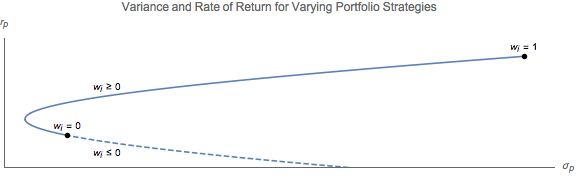
\includegraphics[width=5in, height=2in]{figures/stocks.png}
\end{figure}

We then covered two more things -- the triangle plot and the efficient frontier graph. These should probably be included in the notes at some point. The essential idea is that, as more stocks are included, you decrease the risk and increase the reward. 

\subsection{Markowitz Model}
The Markowitz model can be defined as a functional in which we attempt to minimize $\sigma_{ij}$ by defining $w_i$ and $w_j$ such that
$$\mathcal{L} = \sum \sum w_i w_j \sigma_{ij} - \lambda(\sum w_i \bar{r}_i - \bar{r}_p) - \mu (\sum w_i - 1)$$
Note that in this case we aren't allowing shorting -- that's why we have a $\mu$ coefficient. We can start small by solving the Lagrangian with only two weights, $w_1$ and $w_2$. We have that $$2w_1 \sigma_1^2 + 2 \sigma_{12}w_2 - \lambda \bar{r}_1 - \mu = 0$$ and $$2 \sigma_{21} w_1 + 2\sigma_2^2 w_2 - \lambda \bar{r}_2 - \mu = 0$$subject to the constraints $w_1 \bar{r}_1 + w_2 \bar{r}_2 = 1$ and $w_1 + w_2 = 1$. Solving these equations yields $w_1 = - (r_2 - r_p) / (r_1 - r_2)$ and $w_2 = - (r_p - r_1) / (r_1 - r_2)$. 
\example Given three stocks in which $\sigma_i^2 = 1$ and each stock is uncorrelated with the rest (the $\sigma$ term between the stocks is 0), and $r_i = i$, find $r_p$ and $\sigma_p$ of the portfolio. We're again optimizing the same functional, and taking the individual derivatives yields 
\begin{align*}
2w_1 - \lambda - \mu &= 0 \\
2w_2 - \lambda - \mu &= 0 \\
2w_3 - \lambda - \mu &= 0 \\
w_1 + 2w_2 + 3w_3 &= r_p \\
w_1 + w_2 + w_3 &= 1
\end{align*}
which resolves to $r_p = 2+\lambda$, $w_1 = 2+\lambda$, $w_2 = 1/3$, $w_3 = 1/3 + \lambda/2$, and $\mu = 2/3 - 2\lambda$. We've therefore solved for $r_p$; our next task is to find $\sigma_p$. We can do this by noting that $\sigma_p^2 =w_1^2 + w_2^2 + w_3^2$ (as $\sigma_p$ is the square root of the covariance term). If we replace $\lambda = r - 2$, this resolves to $\sigma_p = \sqrt{7/3 - 2r + r^2/2}$. At the vertex ($-b/2a$ for a quadratic), we have $r = 2$ and $\sigma_p = 1/\sqrt{3}$.   
\subsection{Two Fund Theorem}
We know our $\sigma$ versus $\bar{r}$ graph for $n$ stocks looks like the graph depicted above. If we have two points (defining the two funds), we can characterize Fund 1 by $w^1 : (w_1', w_2', \dots w_n')$ with $\lambda^1, \mu^1$, and $r^1$. and Fund 2 by $w^2 : (w_1', w_2', \dots w_n')$ with $\lambda^2, \mu^2$, and $r^2$. We can form a combination of these two funds $$\bar{r} = \alpha w^1+ (1-\alpha)w^2$$where $\alpha$ is any number. This defines all of the points on the efficient frontier; so if we have two optimal funds all we have to do is invest in those two funds with a varying $\alpha$. More formally, two efficient funds can be established so that any efficient portfolio can be duplicated in terms of the mean-variance as a combination of these two. All investors seeking efficient portfolios need only invest in a combination of two funds. 

\subsection{Inclusion of a Risk-Free Asset}

A risk-free asset has a fixed return and $\sigma = 0$. We can define our return as as $\bar{r} = \alpha r_f + (1-\alpha) \bar{r}_p$ (where $r_f$ is the risk-free asset return and $\bar{r}_p$ is the return of the $n$ risky assets), and $\sigma = \alpha \sigma_f + (1-\alpha) \sigma_p$. It turns out that, with a risk free asset, our frontier is a line with a $y$-intercept at $r_f$ (because $r_f$ has no risk) that is tangent to the risky asset frontier. The single-fund theorem states that, given $F$ is a single fund of risky assets, any efficient portfolio can be constructed as a combination of the fund $F$ and the risk free asset. 

\subsection{One Fund Theorem}
Say we have a combination of risky assets and a risk free bond: what is our efficient frontier for investments between the two? We start by drawing the efficient frontier for an imaginary "extra" stock that is some linear combination of investments in all possible risky stocks. We then draw a line from the rate of the risk free asset, $r_f$, to a point tangent on the risky efficient frontier that maximizes the angle $\theta$ between the line and the horizontal called $F$. A straight line between the point $r_f$ on the risk-free asset and the tangent on the risky frontier becomes our new efficient frontier for the combination of the risky and risk free assets.

\proof Suppose we have $n$ risky assets and weights $w_1, w_2, \dots w_n$ such that $\sum w_i = 1$. We note that at point $F$, zero weight is put on the risk free $r_f$. Note the following definitions:
$$r_p = \sum w_i R_i$$
$$\bar{r}_p = \sum w_i \bar{r}_i$$
$$r_f = \sum w_i r_f$$
\begin{align*}
	\tan{\theta} 	&= \frac{\bar{r}_p - r_f}{\sigma_p}\\
				&= \frac{\sum w_i(\bar{r}_i - r_f)}{(\sum \sum \sigma_{ij} w_i w_j)^{\frac{1}{2}}}
\end{align*}
We can set up the following inequality through Lagrangian optimization of the angle $\theta$ subject to the weights summing to one, yielding
$$\sum \sigma_{ki} \lambda w_i = \bar{r}_k - r_f$$
We define a new quantity $v_i$ to be $\lambda w_i$. Rewriting the equation yields that
$$\sum_i \sigma_{ki} v_i = \bar{r}_k - r_f$$
$$w_i = \frac{v_i}{\displaystyle \sum_k v_k}$$ 

\subsection{CAPM}
Markowitz had two primary tenets in his theory: how should one invest one's money and how much is a security really worth? Under the former part, one attempts to minimize risk for a given rate of return using quantities like random variables, means, standard deviations, and covariances. Under the second portion, new theory is required:
We can rewrite the expected rate as
$$r_i = \frac{Q_i}{P_i} - 1$$
where $P_i$ is the current stock price and $Q_i$ is the stock price a year from now. While $P_i$ is a constant, $Q_i$ is a random variable. We can also define return and risk as of a security as
\begin{align*}
\bar{r}_i &= \frac{\mathrm{E}[Q_i]}{P_i} - 1\\
\sigma_i &= \frac{\mathrm{SD}[Q_i]}{P_i}
\end{align*}
But what if instead of one Markowitzian investor we had $m$ of them. What would the new equilibrium price of the stock become? We'll need to use the basic economic laws of supply and demand. On the demand side, each investor has a budget $B_j$ ($j = 1, 2, \dots m$).  Given $P_i$ ($i = 1, 2, \dots m$), the investor will find their optimal mixed portfolio and issue orders to buy and sell. On the supply side, the number of shares is a fixed $K_i$ ($i=1,2,\dots, m$). If someone wants to buy a stock, someone else must be willing to sell one.

Assume we have some "magic stock" $M$, which acts as a point on the efficient frontier mixed with a risk free security $r_f$. If $M$ is efficient, then the expected return $r_i$ of any asset $i$ satisfies 
$$\bar{r}_i - r_f = \frac{\sigma_{iM}}{\sigma_{M}^2}(\bar{r}_M - r_f)$$

\proof Consider a portfolio with $\alpha$ invested in asset $i$ and 1 - $\alpha$ invested in $M$.
Consider the following definitions:
\begin{align*}
\displaystyle \bar{r}_\alpha &= \alpha \bar{r}_i + (1 - \alpha) \bar{r}_M\\
\displaystyle \sigma_\alpha &= \sqrt{\alpha^2 \sigma_i^2 + 2\alpha(1-\alpha)\sigma_{iM} + (1 - \alpha)^2 \sigma_M^2}
\end{align*}

$\alpha$ being equal to zero is equivalent to investing entirely in M.

\begin{align*}
\frac{\mathrm{d}\bar{r}_\alpha}{\mathrm{d}\alpha} &=  \bar{r}_i - \bar{r}_M\\
\frac{\mathrm{d}\bar{\sigma}_\alpha}{\mathrm{d}\alpha} &= \frac{\alpha \sigma_i^2 + (1 - 2\alpha)\sigma_{iM} + (\alpha - 1)\sigma_M^2}{\sigma_\alpha}\\
\frac{\mathrm{d}\bar{\sigma}_\alpha}{\mathrm{d}\alpha}\biggr\rvert_{\alpha = 0} &= \frac{\sigma_{iM} - \sigma{M}^2}{\sigma_M}\\
\frac{\mathrm{d}\bar{r}_\alpha}{\mathrm{d}\sigma_\alpha} &= \frac{(\bar{r}_i - \bar{r}_M)\sigma_M}{\sigma_{iM}-\sigma_M^2}\\
 \frac{(\bar{r}_i - \bar{r}_M)\sigma_M}{\sigma_{iM}-\sigma_M^2} &= \frac{\bar{r}_M - r_f}{\sigma_M}
\end{align*}
Solving for $\bar{r}_i$ yields that $\bar{r}_i = r_f + \frac{\bar{r}_M - r_f}{\sigma_M^2} \sigma_{iM}$
\begin{align*}
r_i &= \frac{Q_i}{P_i} - 1\\
\frac{\mathrm{E}[Q_i]}{P_i} - 1&= r_f + \frac{\sigma_{iM}}{\sigma_M^2}(\bar{r}_M - r_f)\\
P_i &= \frac{\mathrm{E}[Q_i]}{1 + r_f + \frac{\sigma_{iM}}{\sigma_M^2}(\bar{r}_M - r_f)}\\
\frac{\sigma_{iM}}{\sigma_M^2} 	&= \frac{\mathrm{Cov}[(\frac{Q_i}{P_i} - 1), r_M]}{\sigma_M^2}\\
							&= \frac{\mathrm{Cov}[(Q_i, r_M]}{P_i \sigma_M^2}
\end{align*}
\newpage
\section*{Appendix A---Quotes}
\begin{itemize}
\item ``I have a problem. It's called gambling.'' (Dr. Aiyer)
\item ``What's $E$? Entropy?'' (David Zhu)
\item ``So is it the strong law of weak numbers?'' (Jerry Chen)
\item ``It's like a half life... but it's a double life'' (Steven Cao)
\item ``Isn't this just Lagrange?''  \\ 10 minutes later.. \\ ``Wait, how do you do Lagrange again?'' (Swapnil Garg)
\item ``I'm just amazed that you manage to learn something'' (Dr. Aiyer)
\item (Looking at $\Sigma$) That's a backwards $\xi$! (Steven)
\item ``What's a binomial distribution?'' (Dr. Aiyer) \\ ``$a + bx$'' (Shaya)
\item ``An approximation of $\ln(1-x)$ is $1 + x + x^2 + x^3 + \dots$'' (Misha Ivkov)
\item ``Where does $\epsilon$ go to get a haircut?'' \\ ``The epSALON'' (Shaya)
\item ``So the sample mean is $\hat{\mu}$...'' (Manan Shah)
\item ``Yes, $e^{1/2}$ on most days is $\sqrt{e}$...'' (Dr. Aiyer)
\item ``We're going to try to finish this today (Ha!)'' (Dr. Aiyer)
\item ``Why are we using a $\times$ for multiplication in 2017?'' \\ ``I thought we were at the age where we didn't have to use anything...'' (Rajiv Movva)
\item ``Why do we discuss confidence intervals instead of regions in statistics?'' (Dr. Aiyer) \\ ``We approximate the ellipse to a square'' (Shaya)
\item ``Hey, hey, Rajiv has allrajivs (allergies)" (Vedaad) \\ 	``I thought about that, but I figured it was too bad to say" (Shaya) \\ ``You should never Shayaway (shy away) from a pun" (Misha).
\item Tuesday, March 21, 2017 -- Vedaad came to class \textit{early}.
\item ``We're not in geometry! We don't worry about how to actually do stuff; we just talk about it.'' (Rajiv)
\item Steven: ``Is this a law? (referring to the 2nd law of thermodynamics)'' \\ Rajiv: ``So what's the penalty if you break the law?''
\item (During period 1) Jerry: ``It's been a rough day.'' 
\item ($m^2/4$ is the answer). Manan: ``I got $m^2/2 - m^2/4$...what am I doing wrong?''
\item ``Using good markers changes the lives of students'' (Rajiv)
\end{itemize}
\end{document}
